\subsection{Geologic history}

The geologic history of Mars provides key constraints on interior evolution. The cratering record shows that much of the crust formed very early in Martian history.  Both the hemispheric dichotomy between the southern highlands and northern lowlands and the huge Tharsis volcanic complex provide important constraints on interior structure and evolution. 

Impact crater density is used to divide the history of Mars into fours periods  (see \cite{Werner2011} 2011 for discussion and possible alternate dates): Pre-Noachian (\textgreater 4.1 Ga), Noachian (4.1-3.8 Ga), Hesperian (3.8-3.0 Ga), and Amazonian (\textless 3.0 Ga).  Much of the crust is Hesperian or older, making Mars an ideal location to study initial crustal formation.  The largest impact basins have locally excavated the crust.  The Hellas and Isidis basins are similar in size (see Figure \ref{fig:topo}), but have very different depths and gravity signatures due to subsequent filling of Isidis \citep{Searls2006}. The largest basin, Utopia, is located in the northern plains and is completely buried.  As discussed below, the entire northern hemisphere may have formed as a result of a very early impact, or via endogenic processes. High resolution topography revealed numerous impact basins buried under 1-2 km of fill in the northern plains, implying formation in the Pre-Noachian \citep{Nimmo2005, Frey2006}. Younger, Amazonian age features consist of polar cap ice deposits, volcanism, sediments, and impacts. The InSight landing site in Elysium Planitia, is located near some of the youngest volcanic and tectonic features on the planet \citep{Vaucher2009, Burr2002}, potentially providing seismic sources \citep{Roberts2012, Taylor2013}.
The most prominent topographic features are the dichotomy between the northern and southern hemispheres and the Tharsis volcanic rise. Each of these features are clearly visible in the topography of Mars (Figure \ref{fig:topo}), and relate directly to interior processes or crustal structure.

\begin{figure}[h!]
\begin{center}
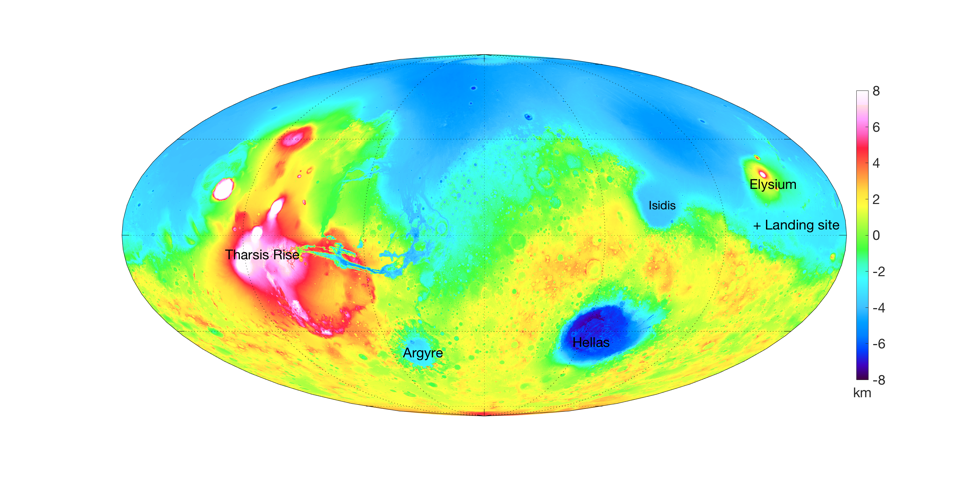
\includegraphics[width=0.85\textwidth]
{figures/Fig_2New.png}
\caption{Key topographic features on Mars include the hemispherical dichotomy, separating the northern lowlands from the southern highlands, the Tharsis volcanic complex, and major impact basins, as labeled.}
\label{fig:topo} 
\end{center}
\end{figure}

The southern highlands are on average 4-5 km higher than the northern lowlands (Figure \ref{fig:topo}), and have a much higher crater density due to infilling of the northern plains by volcanism and sediments. The origin of dichotomy has been attributed to both endogenic processes such as hemispherical scale (degree 1) mantle convection \citep{SCHUBERT1973,Wise1979a,Wise1979, Breuer1997, Breuer1998, Zhong2001} or very early plate tectonic \citep{Sleep1994}. Exogenic models include single \citep{Wilhelms1984} or multiple \citep{Frey1988} impact events. In some scenarios, a degree-1 plume formed under the southern hemisphere and caused massive melting that thickened the crust and produced higher elevation in the south via isostatic adjustment \citep{Zhong2001}.  Alternatively, a degree-1 plume may have thinned the crust in the northern lowlands \citep{Roberts2006}. Another proposed mechanism is the overturn of a buoyantly unstable mantle following magma ocean solidification \citep{Elkins-Tanton2008}. \citep{Andrews-Hanna2008} proposed that the northern plains were formed via a single impact that created an elliptical basin, as predicted by modeling\citep{Marinova2008}. They used both gravity and topography to remove the signature of Tharsis and Arabia Terra on the shape of the northern plains. 

These models have different implications for the composition and structure of the interior. A major question has been whether there is a difference in crustal composition between the north and the south that contributes to the difference in elevation.  A recent investigation of the northern lowlands basement composition, as revealed by impact crater excavations, finds a range of hydrated minerals beneath the surficial volcanic fill, similar in composition to those found in the southern highlands \citep{Pan2017}. Although the sampling depth is limited, this work strongly suggests that the difference in elevation reflects a difference in crustal thickness rather than composition.  Another puzzling question is why the northern lowlands exhibit very little crustal remnant magnetization relative to the southern highlands despite their similarity in age e.g. (e.g.,\cite{Langlais2004}).  One possible explanation is that the dynamo on Mars was asymmetric \cite{Stanley2008}.

Mars’ other major physiographic feature is the Tharsis rise, a massive volcanic complex.  It covers one quarter of the Martian surface and is the largest volcanic construct in the solar system (Figure \ref{fig:topo}).  The rise itself is ~10 km high, with three central volcanoes with heights of \textgreater 10 km each, in addition to Olympus Mons to the northwest and Alba Patera to the north (Figure \ref{fig:topo}).  This huge feature affects the global topography, gravity, and surface deformation  (see \citep{GolombekM.P.andPhillips2009PlanetaryTectonics}for a review). The age of the planetary scale deformation associated with Tharsis and the extensive volcanism indicate that the region has been active over most of the age of Mars. Although much of the topography is interpreted to have formed early in Martian history, modest volcanism persisted into the Amazonian.  For example, Arsia Mons may have been active as recently as 10-90 Ma \cite{Richardson2017}.  

The massive topography of Tharsis must be held up by some combination of compositional and/or thermal isostasy, flexure, and dynamic mantle support.  The exact proportion and origin of these mechanisms have implications for interior structure, mantle dynamics, and thermal evolution.  Models of loading of the lithosphere in response to Tharsis volcanism show that membrane stresses are capable of supporting the majority of the load \cite{Banerdt1982, Banerdt1992} and successfully predict more deformation features than isostatic models, even if coupled with a regional stress field \citep{Tanaka1991}.  Much of the lithospheric deformation dates to the Middle Noachian (\textgreater 3.8 Ga), and requires that the Tharsis load have the dimensions of the current topographic rise \cite{Phillips2001}.  Modeling of the present-day gravity and topography fields also predict the pattern of deformation, indicating that the stress fields have largely been unchanged since the Noachian \cite{Banerdt2000}. \citet{Bouley2016} proposed an alternative explanation, suggesting that the orientation of a key deformation feature, valley networks, can be explained by topographic gradients between the northern and southern hemispheres prior to Tharsis formation. In this scenario, major Tharsis construction begins in the Late Noachian.  One question for these loading models and interior structure is the degree of support due to low density mantle residuum \cite{Phillips1990}.

The Tharsis rise has been interpreted as forming over one or more mantle plumes.  The scale of plume, the formation of most of the volcanism early in Martian history, and the continuation of volcanic activity into recent Martian geologic history, have posed a challenge for convection simulations.  A series of convection models have shown that the presence of a phase transition near the core-mantle boundary supports the formation of a small number of plumes and areal concentration of plumes \citep{Harder1998,Harder2000,Harder1996,Breuer1998}. The size of the core is the dominant factor in determining whether or not phase transitions near the core-mantle boundary are present, and thus the applicability of such plume models. Another key challenge is for the convection pattern to localize rapidly enough to be consistent with timing constraints on the formation of Tharsis.  A key question is source of relatively recent volcanism given the very thick lithosphere under Tharsis. Modeling suggests that if present, a plume or other buoyant region at depth contributes only modestly to support of the topography \citep{Lowry2003,Zhong2003, Roberts2004, Redmond2004} Redmond and King, 2004).  Alternative ideas for the formation of Tharsis include warming of the mantle \cite{Solomon1982a}.  Warming might occur under a thick, insulating southern hemisphere crustal layer \cite{Wenzel2004}. 

\subsection{Composition}
Our current knowledge of the bulk chemical and mineralogical composition of Mars is based on the analysis of the Martian meteorites, remote sensing and in-situ analysis of the Martian surface as well as on geophysical properties of the planet.   

\subsubsection{Meteorites, remote sensing and in-situ analysis}
Martian meteorites partially referred to as SNC meteorites (shergottites, nakhlites, and chassignites) are igneous rocks of varying mafic to ultramafic igneous lithologies. The meteorites exhibit both intrusive and extrusive textures including: basalt and lherzolite (shergottites), orthopyroxenite (ALH 84001), clinopyroxenite (nakhlites), and dunite (Chassigny). Except for ALH 84001, a 4.5-Ga sample of the Noachian crust, all SNCs were extracted from Amazonian volcanic terrains. The most representative samples are the shergottites that show crystallization ages between 170 and 600 Ma (e.g., McSween and McLennan, 2014).  For characterizing the chemistry and mineralogy of igneous materials at the surface of Mars, remote sensing data are also available. Mineralogical information is generally obtained using the visible and infrared range of the electromagnetic spectrum \citep{Bandfield2000, Poulet2009}, whereas abundances of chemical elements are principally derived from gamma-rays \citep{Boynton2007} and neutron spectroscopy (Feldman et al. 2011). In general, the spectral analysis of the Martian surface does not provide a good match to the spectral signature of the SNC meteorites \cite{HAMILTON2003, Lang2009} and Martian meteorite-like lithologies represent only a minor portion of the dust-free surface. However, the distinctive mineralogical characteristics of SNCs (ferroan olivine and pyroxenes, sodic plagioclase) are commonly indicated by remote-sensing data. Igneous rocks have also been analyzed in-situ in both Gusev Crater (e.g.,\cite{Squyres2004}). These rocks also range from basaltic to cumulate rocks (e.g.,Dreibus et al., 2007; McSween et al., 2006; Ming et al., 2008; Squyres et al., 2006) but are much older (\textasciitilde 3.65 Ga) than shergottites \citep{Arvidson, Greeley2005} and have significantly different chemistry than basaltic shergottites (Filiberto et al., 2006; \citep{McSween2009}; Taylor et al., 2006). These findings challenge the use of the SNCs in defining diagnostic geochemical characteristics and in constraining compositional models for Mars. We also note that extensive sedimentary deposits composed of phyllosilicates and sulfates have been observed from orbit and by rovers in Gale crater and Meridiani Planum, but spectral data from orbit (Ehlmann et al. 2011; Ehlmann and Edwards. 2014) and chemical and mineralogical data from the surface \cite{DavisA.M.McSweenH.Y.Jr.&McLennan2005} Grotzinger et al. 2014) show that most are basaltic in composition or have been altered from an initial basaltic composition, indicating that the martian crust is basaltic in composition.

\subsubsection{Bulk composition}
\setcounter{tocdepth}{4} \setcounter{secnumdepth}{4}
\paragraph{Geochemical perspective}

Assuming that the SNC meteorites are representative of the Martian crust, models based on geochemical arguments \cite{Dreibus1984}\cite{Dreibus1984AccretionPlanets.,Dreibus&Wanke1985, Wanke1994, Lodders1997, Morgan1979, Sanloup1999}. \cite{Mohapatra&Murty2003} have been developed to estimate the composition of the bulk silicate portion of Mars (see Taylor, 2013, for a recent review). To derive the chemical composition of Mars from the chemical compositions of the Martian meteorites, two general approaches have been applied. The first approach uses the elemental correlations in the Martian meteorites, assuming that refractory elements are present in chondritic abundances \cite{Dreibus1984, Dreibus1984AccretionPlanets.,Dreibus&Wanke1985, Wanke1994, Halliday2001, Longhi1992, Taylor2013} whereas the second approach uses oxygen isotope systematics of the SNC meteorites and match them via mass balance equations to mixtures of different chondritic material \citep{Lodders1997,Sanloup1999, Burbine2004}. Table \ref{compositiontable} shows a compilation of 5 different models of the bulk composition of Mars. These compositions represent the primitive mantle of Mars, i.e., unaffected by magmatic processes such as magma ocean fractional crystallization and crust formation. 

\begin{table}[h!]
\centering
\label{comptable}
\begin{tabular}{lllllll}
                                                & MA    & DW    & LF    & SA    & TA   &  \\
                                                &       &       &       &       &      &  \\
Bulk crust \& mantle composition(wt.\%) 
in major oxides &       &       &       &       &      &  \\
\ce{SiO2}                                            & 41.59 & 44.4 & 45.39 & 47.79 & 43.7 &  \\
\ce{Al2O3}                                          & 6.39  & 3.02  & 2.89  & 2.52  & 3.04 &  \\
MgO                                             & 29.77 & 30.2 & 29.71 & 27.46 & 30.5 &  \\
CaO                                             & 5.16  & 2.45  & 2.36  & 2.01  & 2.43 &  \\
\ce{Na2O}                                            & 0.1   & 0.5  & 0.98  & 1.21  & 0.53 &  \\
\ce{K2O}                                            & 0.01  & 0.04  & 0.11  & -     & 0.04 &  \\
\ce{TiO2}                                            & 0.33  & 0.14  & 0.14  & 0.1   & 0.14 &  \\
\ce{Cr2O3}                                           & 0.65  & 0.76  & 0.68  & 0.7   & 0.73 &  \\
MnO                                            & 0.15  & 0.46  & 0.37  & 0.4   & 0.44 &  \\
FeO                                             & 15.85 & 17.9 & 17.21 & 17.81 & 18.1 &  \\
                                                &       &       &       &       &      &  \\
Core composition                                &       &       &       &       &      &  \\
Fe                                              & 88.1  & 77.8  & 81.1  & 76.6  & 78.6 &  \\
Ni                                              & 8     & 7.6   & 7.6   & 7.2   &      &  \\
S                                               & 3.5   & 14.2  & 10.6  & 16.2  & 21.4 & 
\end{tabular}
\caption{Bulk Martian crust and mantle (primitive mantle) and core composition for model MA \cite{Morgan1979}, DW  \cite{Dreibus1984},\citep{Wanke1994}, LF \citep{Lodders1997}, SA \citep{Sanloup1999} and TA \citep{Taylor2013}}.
\label{compositiontable}
\end{table}

All compositional models share the characteristic that the Martian mantle is more Fe-rich than the Earth, consistent with the Fe-rich compositions of SNC meteorites.  The significant difference between oxygen isotope-based and element-based estimates is the strong enrichment in volatile elements in the isotope models. This enrichment is not seen in the GRS data \citep{Taylor2007} for which K/Th is 5300 for the Martian surface versus K/Th 16400 in the study of \citep{Lodders1997}. The model by \citep{Wanke1994}, recently reassessed by Taylor (2013) using a larger meteoritic record, is broadly consistent with the surface K/Th ratio measured by the GRS instrument \citep{Taylor2007BulkMars} and is currently the most widely accepted compositional model.  

It should be noted that although Martian meteorites are an important data set, element abundances in the crust derived from in-situ and remote sensing measurements suggest that magma source regions are heterogeneous and constraints on mantle compositional models from the meteorites may not apply to the entire mantle. In addition, the isotope characteristics of the SNCs indicate the formation of several reservoirs, which have formed rapidly in the first ten million years after the formation of the planet and have not been mixed since then (e.g.\cite{Mezger2013}). An aspect that is difficult to take into account in current models of internal structure, since the size and location of these reservoirs are unknown – thus typically a chemically homogeneous mantle is assumed.

\setcounter{tocdepth}{4} \setcounter{secnumdepth}{4}
\paragraph{Geophysical perspective}

Geophysical analyses typically rely on results obtained from the geochemical studies to predict the geophysical response of these models. In particular, many of the geophysical and experimental approaches are based on the \cite{Dreibus1984}  model composition with the purpose of determining mantle mineralogy \citep{Bertka1997, Bertka1998}. Combined with equation-of-state (EOS) modeling allows for determination of a model density profile that can used for making predictions and be compared to observations (e.g., mass, moment of inertia, and tidal response). Many numerical approaches have also been conducted \citep{Longhi1992,Kuskov,Mocquet1996,Sohl1997, Sohl2005,Verhoeven2005,Zharkov2005,Khan2008,Rivoldini2011,Wang2013} Khan et al., 2017).
These studies are based on forward/inverse modeling of the available geophysical observations using either parameterized phase diagram or phase equilibrium computations. These studies generally concur with the geochemical evidence for an Fe enriched Martian mantle relative to Earth’s magnesian-rich upper mantle \cite{McDonough1995}. 

\subsubsection{Mineralogy of the reference models}
The major mineralogical constituents of the mantle are those expected for an Earth-like planet: olivine, ortho- and clino-pyroxenes, and garnets, but in different proportions among the proposed models \citep{Dreibus&Wanke1985,Sanloup1999,Taylor2013,Bertka1997} (Figure~\ref{fig:Fig_Mineralogy.png}). These models show that 1) olivine undergoes phase transitions: to wadsleyite around 12-13 GPa and to ringwoodite at 14-16 GPa; and 2) that pyroxenes progressively transform into garnet solid solutions at depth. The sharpness and the location of these mineralogical transformations mainly depend on the iron enrichment and temperature of the mantle with exothermic transformations occurring at shallower depths in the case of hotter areotherms. Compared to standard Earth-like mantle compositions (e.g., a pyrolitic one), Mars' mantle mineralogy is characterized by the existence of othopyroxenes over a large range of pressure (up to 10 GPa), followed by high-pressure clinopyroxene phases that co-exist with their low-pressure counterparts and with wadsleyite between 10 GPa and 15 GPa.

The existence of a lower mantle as in the Earth is highly dependent on physical conditions at the core-mantle-boundary (CMB), core size and Fe-content. The stability of these silicates is strongly sensitive to temperature and pressure conditions at the CMB: a large core results in either a thin or no lower mantle, whereas higher temperatures will stabilize bridgmanite at lower pressures. Compositionally, small cores will tend to be Fe-rich and favor presence of a lower mantle whereas large cores will tend to be enriched in light elements and inhibit a lower mantle (e.g., \cite{Khan2018}).
\begin{figure}[h!]
\begin{center}
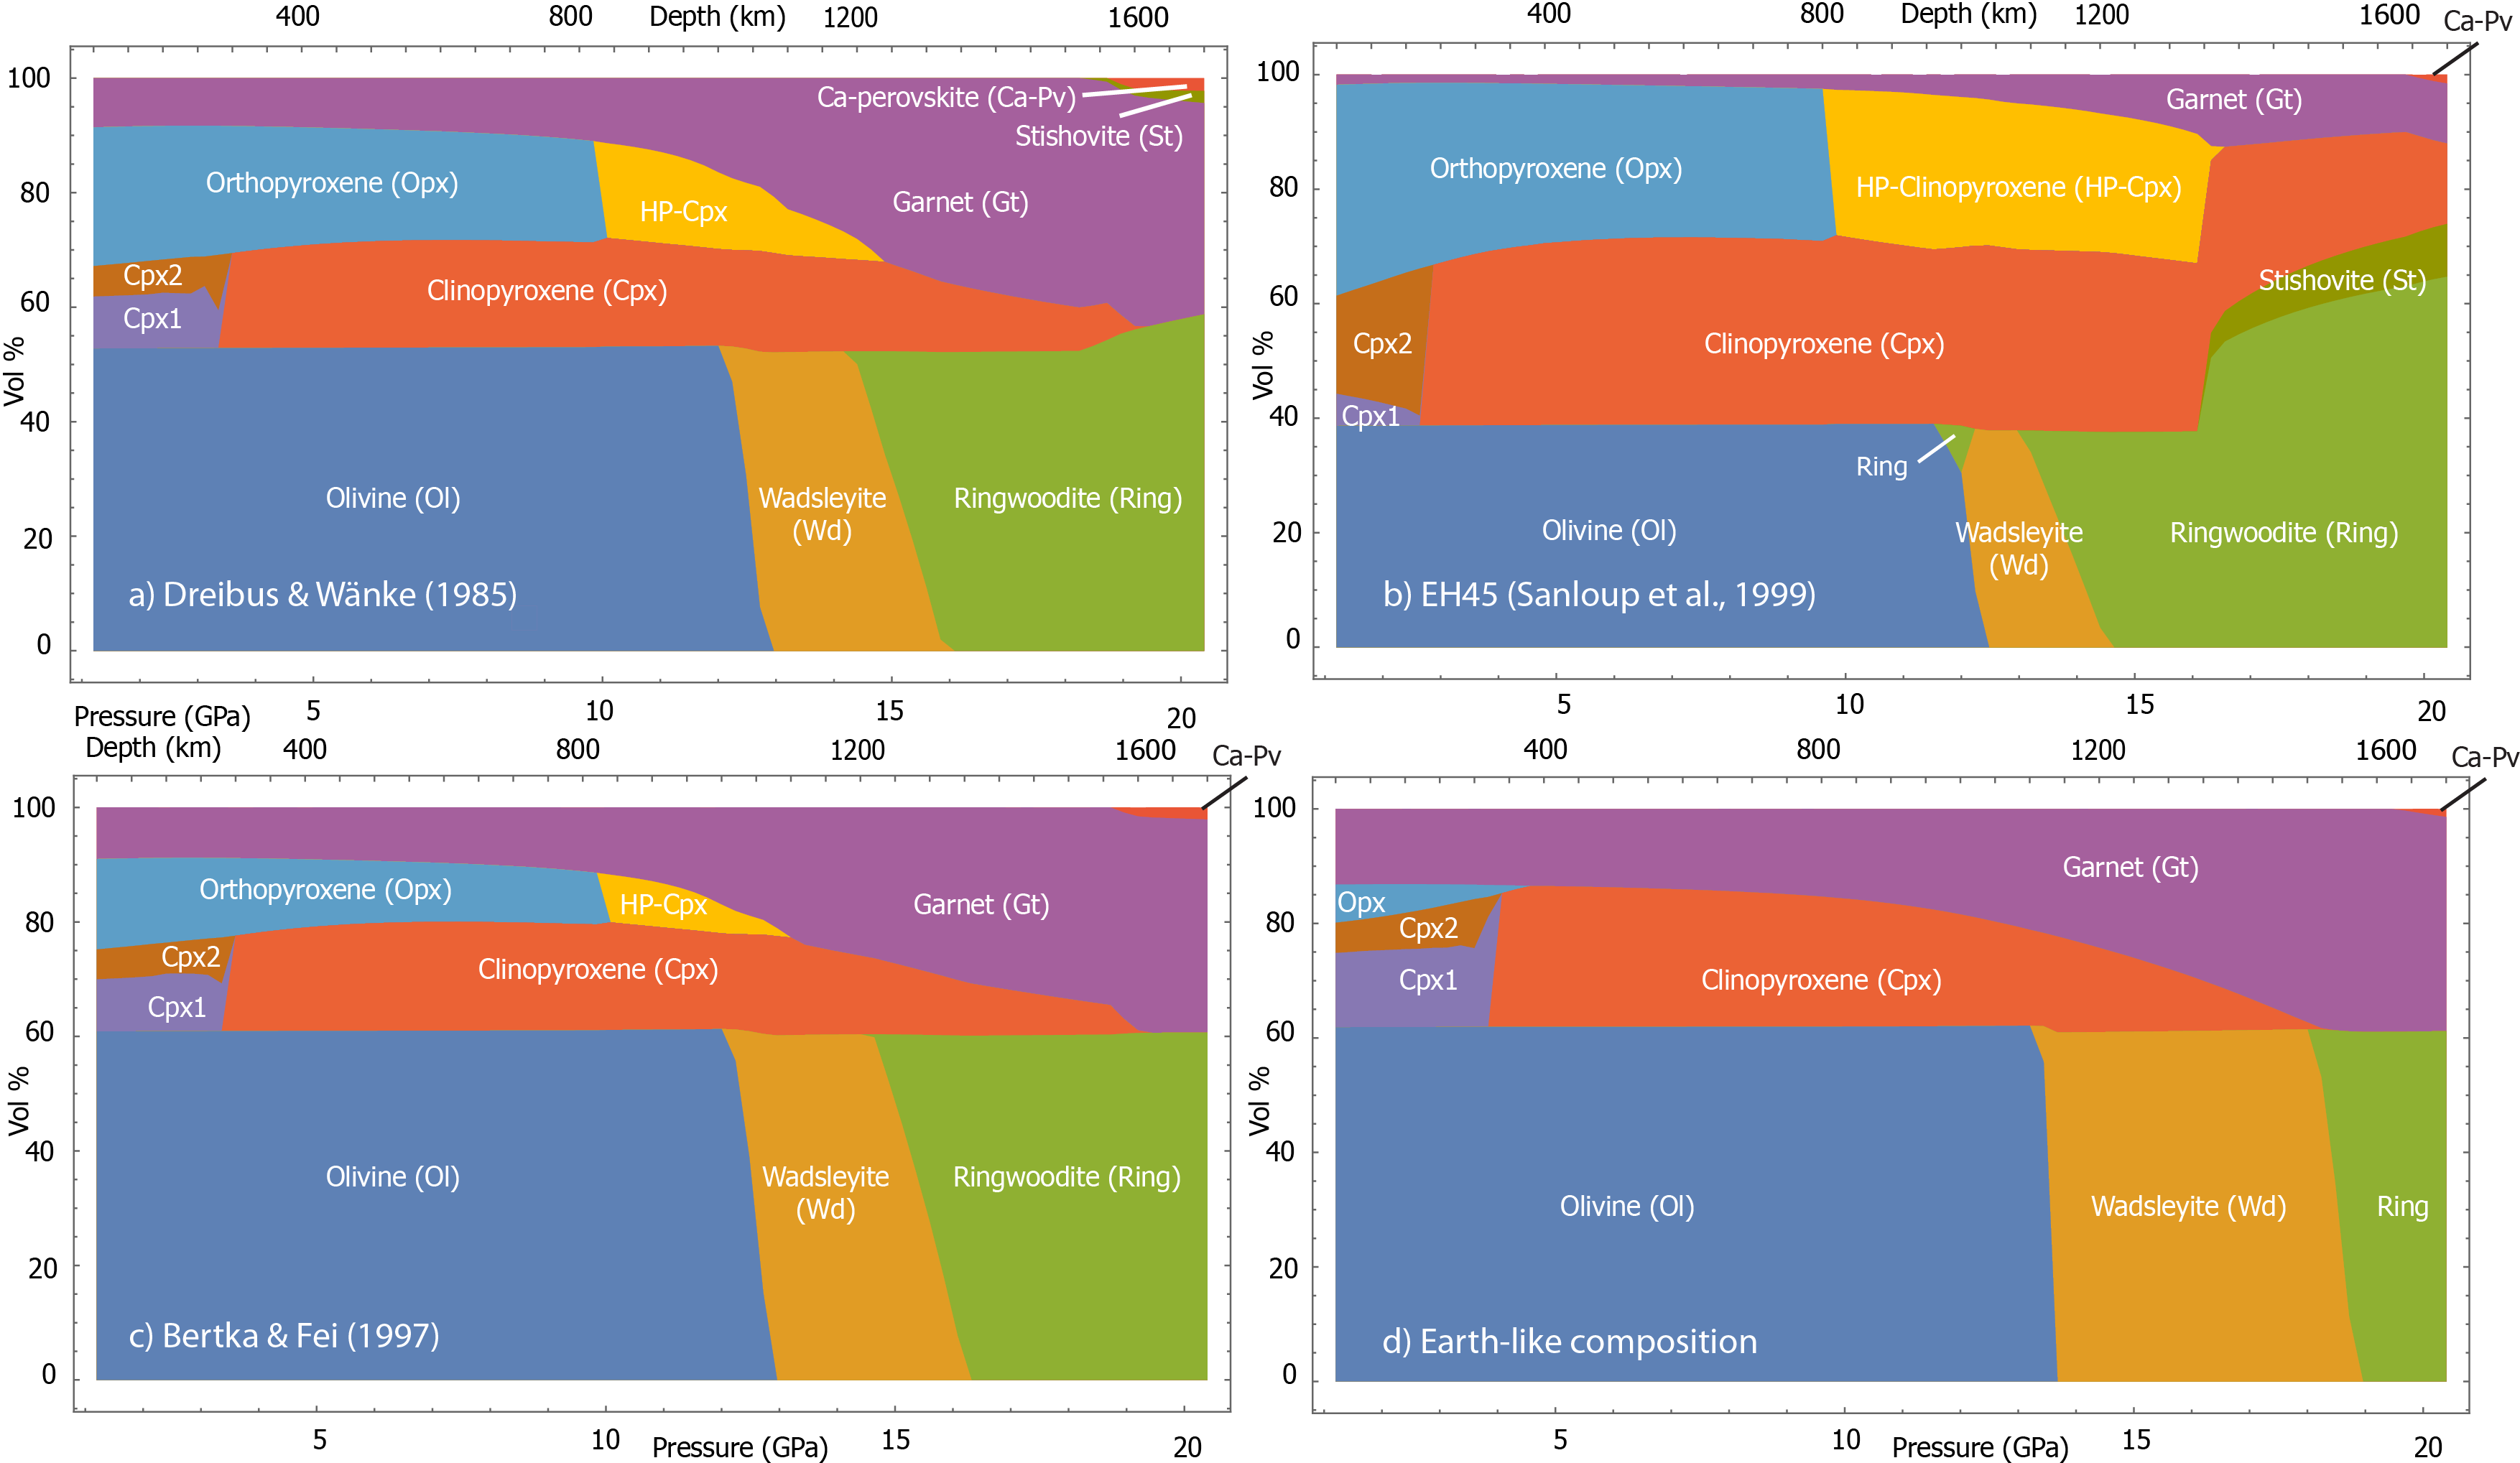
\includegraphics[width=1.0\textwidth]
{figures/Fig_Mineralogy.png}
\caption{Modal mineralogy of Mars as a function of pressure for four bulk compositions. a) Olivine-rich composition of \cite{Dreibus&Wanke1985} revised by \cite{Taylor2013}; b) Pyroxene-rich composition of \cite{Sanloup1999}; c) Modal composition synthetized by \cite{Bertka1997} at high pressure and high temperature. The iron content of the three Martian models (Fe\#0.2) is twice the Earth's mantle value (Fe\#0.1). An Earth-like pryrolitic composition \citep{Ringwood1975} is displayed in panel d) for comparison.}
\label{fig:Fig_Mineralogy.png} 
\end{center}
\end{figure}

\subsection{Gravity, Topography, and Crustal Thickness}

Models of the gravity field of Mars have been improved successively by the analysis of radio tracking data from multiple spacecraft over a time span of several decades. The most recent models (e.g., Genova et al. 2015, Goossens et al. 2017) are expressed up to spherical harmonic degree and order 120, which corresponds to a full-wavelength spatial resolution of about 178 km on the surface. The gravity field is uniquely determined by the three-dimensional distribution of mass within the planet, and thus provides information on how density varies both laterally and with depth. Interpretation of the gravity field is well known to be inherently non-unique, but by making reasonable assumptions based on geologic expectations, and by making use of the surface topography of the planet  (Smith et al. 2001) as a constraint, it is possible to invert for several properties related to the crust and lithosphere.\par
One analysis approach is to assume that Mars differentiated into a distinct crust and mantle, and that the ancient highland crust is isostatically compensated. This model predicts a relationship between the average crustal thickness, the crustal density, and the ratio of the geoid and topography (Wieczorek and Phillips 1997). Mars is divided along a hemispheric dichotomy into the heavily cratered southern highlands and the northern lowlands, where impact basins have been buried by a combination of sedimentation and volcanism. (Wieczorek and Zuber 2004) argue that the southern highlands are more likely to be isostatically compensated than the lowlands. They find that the best-fitting average thickness of the highlands crust was between 53 and 68 km for assumed crustal densities of 2700 and 3100 kg m\textsuperscript{3}, respectively. When considering the uncertainties on the geoid-to-topography ratio, the 1$\sigma$  limits of the average crustal thickness range from 39 to 81 km. The major uncertainty with this approach is that it is difficult to prove that the ancient crust is in fact isostatically compensated, and the density of the crust is highly uncertain.\par

A second modeling approach that can be made is to assume that the rigid outer portion of the planet, the lithosphere, behaves as an elastic shell when subjected to loads both on the surface and within the crust. For a given elastic thickness, these models compute the loads and lithospheric deflections that match the observed surface topography. Though these models depend upon several parameters, including the crustal thickness and mantle density, the density of the surface load is the best constrained. Localized spectral analyses applied to the large Martian volcanoes shows that the densities of the volcanic loads are close to 3200 kg m\textsuperscript{3} \citep{McGovern2004, Belleguic2005, Grott2012}. Beuthe et al. 2012), which are consistent with the densities of the Martian basaltic meteorites \citep{Neumann2004}. Only for the Elysium rise is the density of the crust beneath the volcanic load constrained in these models. For this region in the northern lowlands, the density of the underlying crust was found to be the same as that of the volcanic load itself \citep{Belleguic2005}, suggesting that the entire northern lowland crust may be largely basaltic. The elastic thicknesses obtained from these studies will be discussed in section 3.1.\par
A third modeling approach is to assume that the observed gravitational field is a result of variations in relief along the surface and crust-mantle interface. By assuming densities of the crust and mantle, as well as a mean thickness of the crust, it is possible to invert for the relief along the crust-mantle interface, providing a global crustal thickness map (e.g., \citep{Neumann2004}. This modeling approach makes no assumptions as to whether the crust is isostatically compensated or not, and in practice, the parameter values for the inversions are constrained such that the minimum crustal thickness is equal to a specified value that is greater than zero. The minimum crustal thickness of Mars is found to be located in the interior of the Isidis impact basin, which lies just south of the dichotomy boundary. One of the major uncertainties with these models is that the crustal density is not known. As shown by \cite{Baratoux2014}, the surface composition of Mars is similar to the basaltic meteorites. If these high densities are representative of the underlying crust, to obtain positive crustal thicknesses everywhere, the mean crustal thickness could be as high as 110 km (see also Pauer and Breuer 2008, who provide a maximum density of 3020 kg m\textsuperscript{3}). The minimum crustal thickness to use in these models is also unconstrained, though a value close to zero, as with the Moon (Wieczorek et al. 2013, Miljković et al. 2015), is probably a reasonable estimate. Lastly, it is likely that the density of the subsurface crust varies laterally, but these variations are not easy to constrain based on remote sensing data.

We have constructed a suite of crustal thickness models for use in modeling the seismic data that will be obtained from InSight (see also \cite{Plesa2016}). These models differ from previous studies in several ways. First, in computing the gravity field, we consider the hydrostatic deflection of density interfaces within the mantle and core using the reference density models shown in Section 3.2.3. These models consider the non-hydrostatic gravitational potential arising from the lithosphere when computing the hydrostatic interfaces, and these deflections are responsible for 3.6-5.6\% of the observed zonal degree-2 gravitational field. Second, we consider the possibility that the density of the crust in the northern lowlands is different from that of the southern highlands (e.g., \cite{Belleguic2005}). Third, we consider a wide range of crustal densities, from 2700 to 3200 kg m\textsuperscript{3}. Lastly, as their are yet no seismic constraints on crustal thickness, we use a minimum thickness constraint, where the minimum crustal thicknesses from 1 to 20 km. The thickness of the crust at the InSight landing site varies from 19 to 90 km in these models. In Figure \ref{fig:GravityTopo} , we show one such model where the crustal densities of the southern highlands and northern lowlands are 2900 and 3000 kg m\textsuperscript{3}, respectively. Data obtained from the InSight mission will constrain the crustal thickness at the InSight landing site, and will also constrain the core and mantle density profiles.

\begin{figure}[h!]
\begin{center}
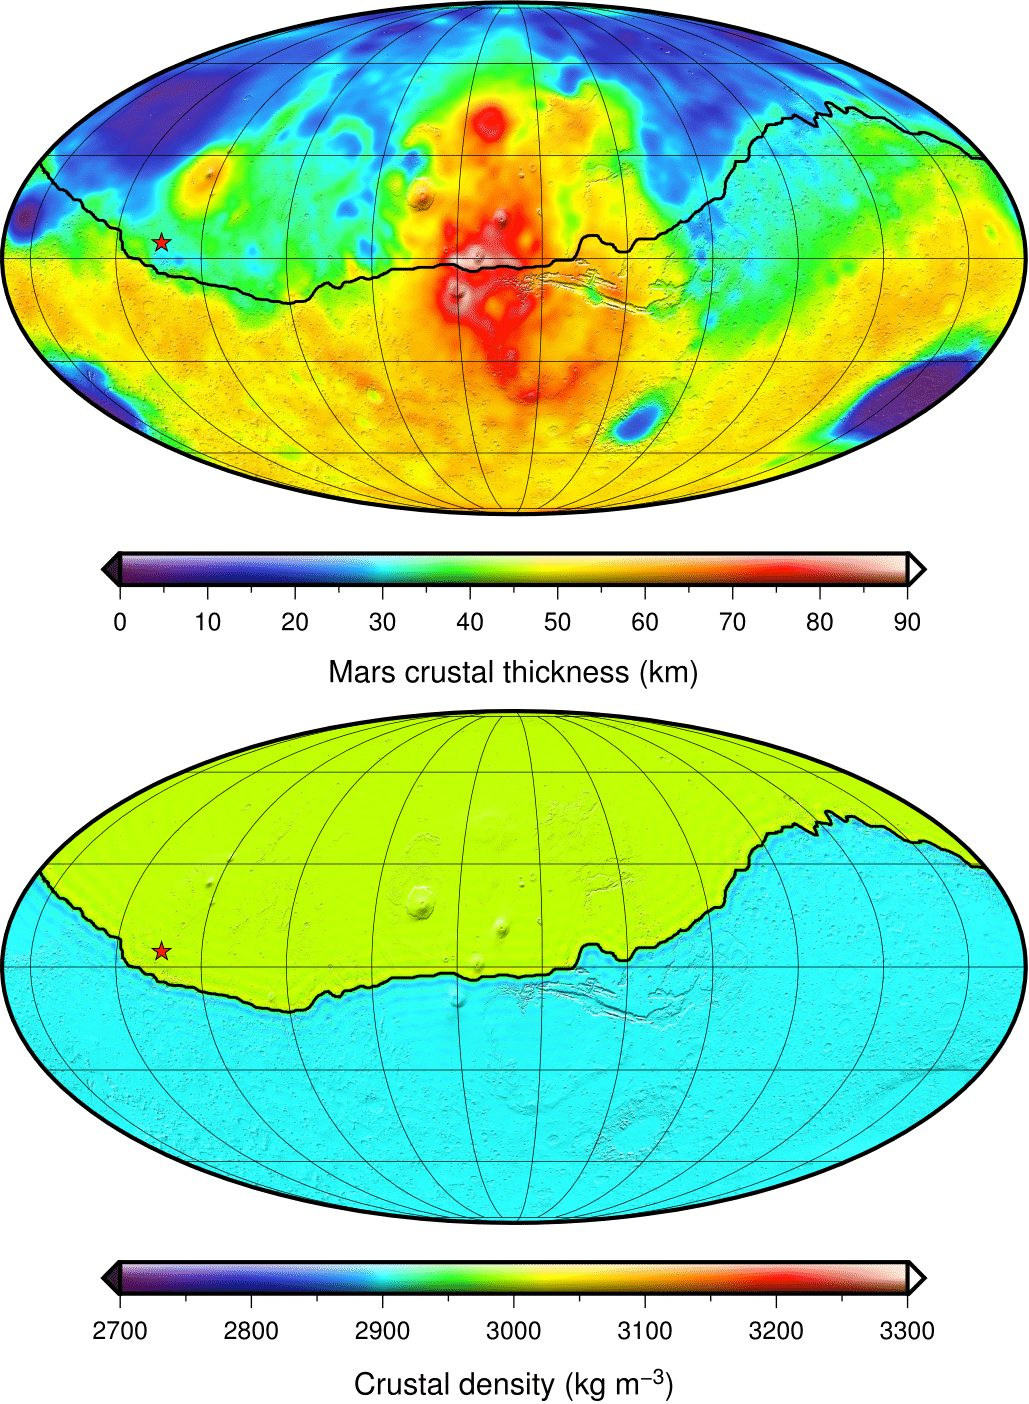
\includegraphics[width=0.65\textwidth]
{figures/GravityTopo.png}
\caption{Representative crustal thickness model (top) using the interior density profile for the model DWTh2Ref1. The crustal densities for the southern highlands and northern lowlands (bottom) are 2900 and 3000 kg m-3, respectively. The minimum crustal thickness was constrained to 1 km, which determines the average crustal thickness to be 42 km and the crustal thickness at the InSight landing site (star) to be 32 km. Data are presented in Mollweide projections centered over the Tharsis province (100° W), and grid lines are spaced every 30 in latitude and longitude. The dictomomy boundary used in the lower image is taken from \citep{Andrews-Hanna2008}}
\label{fig:GravityTopo} 
\end{center}
\end{figure}


\subsection{Constraints on the Lithosphere Thickness}

In the absence of direct heat flow measurements, temperatures in the planetary interior can be estimated from the mechanical properties of lithospheric plates. In this regard, the effective elastic lithosphere thickness Te is commonly used to describe the response of the lithosphere to loading, and given a rheological model, the mechanical thickness of the lithosphere Tm can be derived from Te. Using the yield-strength envelope formalism \citep{McNutt1984}, Tm can in turn be identified with an isotherm, and in this way estimates of planetary heat flow can be derived.

Most Te estimates for Mars have been derived from gravity and topography admittance modeling \citep{McGovern2004, Kiefer2004, Belleguic2005, Hoogenboom2006, Wieczorek2008, Grott2012}, but some geological features allow for more direct approaches. \citet{Phillips2008} have modeled the lithospheric deflection due to polar cap loading, and analysis of rift flank uplift has been used to constrain Te at the Tempe Terra, Coracis Fossae, and Acheron Fossae rift systems \citep{Barnett2002, Grott2005, Kronberg2007}. In addition, the lithospheric stress distribution due to mascon-loading at the Isidis basin has been employed to model Te using the position of the Nili Fossae circumferential graben system as model constraint \citep{Comer1985, Ritzer2009}. Other approaches estimate Te from an analysis of the depth to the lithosphere’s brittle-ductile transition \citep{Schultz2001, Grott2007, Ruiz2009,MUELLER2014100, Egea-Gonzalez2017}, but these approaches carry additional uncertainty. 

To correlate heat flow estimates with time it is usually assumed that the observed paleo-flexure corresponds to the age of the deformed surfaces, and flexure is generally assumed to be frozen-in at the time of loading. However, care must be taken when interpreting these results, as stresses in the lithosphere will decay as a function of time due to viscous relaxation and the true time corresponding to the observed paleo-flexure is generally determined by a competition between loading rate, lithospheric cooling rate, and stress relaxation rate \citep{Albert2000, Brown2000}. In this regard, the elastic thickness estimate by \citet{Phillips2008} is an exception, as the time of loading by the Martian polar caps can be tightly constrained to $<5$ Myr \citep{Phillips2008}.

Elastic thickness has increased with time \citep{GolombekM.P.andPhillips2010,Grott2013,Ruiz2014}. In the Noachian, Te was $< 20$ km. Values quickly increased to $>50$ km during the Hesperian, which can at least partially be attributed to rheological layering \citep{Burov1995, Grott2008, Grott2009}. During the Amazonian Te further increased to $40 <$ Te $< 150$ km on average, and best estimates for the present-day elastic thickness are above 150 km. In particular, the absence of lithospheric deflection due to loading at the north polar cap locally constrains present-day Te to values greater than 300 km at this location \citep{Phillips2008}. Such large present-day elastic thickness values could either imply a sub-chondritic bulk composition in terms of heat producing elements \citep{Phillips2008}, or a large degree of spatial heterogeneity of the mantle heat flow \citep{Phillips2008, Grott2009, Grott2010, Kiefer2009, Plesa2016, Breuer2016}. It is worth noting that some studies assume that the large Te determined for features on the Tharsis rise are representative for the rise itself \citep{Banerdt2000,Phillips2001}. As a consequence, Te would have been much larger and close to 100 km during the Noachian \citep{Zhong2002,Zhong2003}, and regional and global flexure models using Te = 100 km were found to be consistent with the location and orientation of tectonic features \citep{Banerdt2000} and valley networks \citep{Phillips2001}.

\subsection{Geodesy}
Planetary geodesy is one of the primary means for probing the interior structure of planets, in particular when no seismic observations are available. By radio tracking many spacecraft orbiting Mars, an accurate gravity field has been determined over the past decades. Expressed in terms of spherical harmonics, the field is now accurate up to about degree 100 \citep{Konopliv2016, Genova2016}, corresponding to a horizontal surface resolution of about 215 km. Most important for the deep interior of Mars are the lowest degrees. The degree-two components of the gravity field are related to the three principal moments of inertia of Mars, and as such inform on the mass distribution in the planet. Information on the radial density profile can be obtained from the mean moment of inertia, but this quantity cannot be determined form the gravity field alone. By complementing the degree-two components of the gravity field with precession, the mean moment of inertia of Mars has been determined and as such a first constraint on the overall mass distribution inside Mars from center to surface has been obtained.

Precession is determined from analysing radio tracking data of Martian landers and orbiters over several decades (e.g. \citep{Konopliv2011, LeMaistre2013, Kuchynka2014, Konopliv2016}. The most recent estimate of the precession rate of Mars yields a mean moment of inertia normalized by the product of mass and squared radius of Mars of 0.3639 \textpm{0.0001}, with the error mainly due to the error on the precession estimate \citep{Konopliv2016}.  Since it is an integrated quantity over the mass density in Mars, the moment of inertia, even when accurately known, cannot precisely constrain more local properties of the interior such as for example the radius of the core. Even employing the simplifying assumption that Mars were to consist of two equal density layers (the core and the mantle plus crust), the error on the core radius from the moment of inertia constraint would be several hundred km Van Hoolst and Rivoldini 2014). RISE will improve the determination of the precession rate by a factor of two but its effect on the estimate of the core radius is negligible without considering other data.

Up to now, solar tides have been the most constraining geodesy quantity for the core of Mars. Since the tidal potential is accurately known (Van Hoolst et al. 2003), the tides can be interpreted in terms of the reaction of Mars to the gravitational forcing which is very sensitive to the size of a liquid core. Tidal surface displacements have not yet been observed since their amplitude is only a few centimeters at most \cite{VanHoolst2003}, but the mass redistribution inside Mars associated with tidal deformations has an observable effect on the orbital motion of spacecraft around Mars. The tidally induced changes in the external gravitational potential of Mars are described by the Love number k2. The most recent determination of the solar tides yields k2=0.163\textpm {0.008}, based on the estimates of \cite{Konopliv2016} and \cite{Genova2016}. It implies that the radius of the core is about 1788 \textpm{73} km for the SEIS reference models (see Fig. 2.5.1). 

\begin{figure}[h!]
\begin{center}
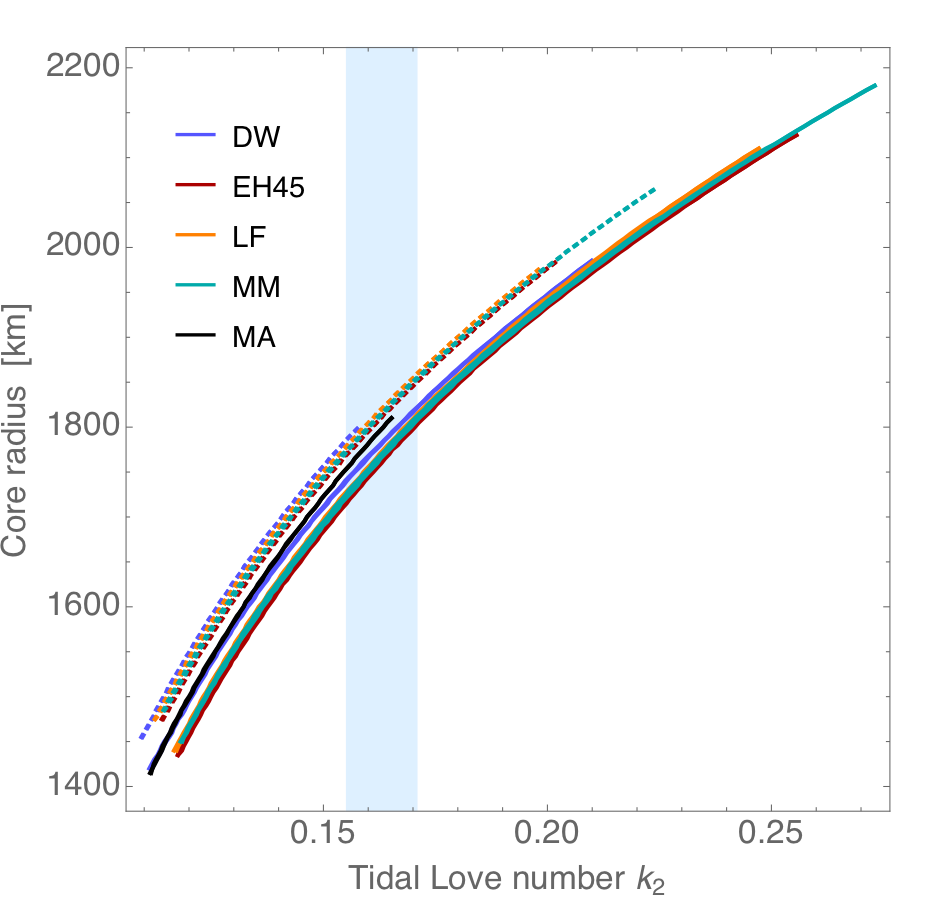
\includegraphics[width=0.65\textwidth]
{figures/Geodesytable.png}
\caption{ Core radius as a function of Love number k2 for the hot (solid curves) and cold (dashed curves) mantle temperature profile from \citep{Panning2016}.  The blue shaded area represents the range of k2 values from \citep{Konopliv2016} and \citep{Genova2016} The acronyms stand for the different mantle mineralogy models (DW: \citep{Taylor2013}, EH45: \citep{Sanloup1999}, LF: Lodders [2000], MM: \citep{Mohapatra&Murty2003}, MA: \citep{Morgan1979}. Models agree at 1$\sigma$ with the average moment of inertia of Mars (MOI=0.3639 \textpm 0.0001) \citep{Konopliv2016}.} 
\label{fig:Geodesytable.png} 
\end{center}
\end{figure}

The radio science experiment RISE of InSight will improve the estimate of precession and thus of the moment of inertia of Mars, but more importantly it will for the first time measure the effect of the core on the periodic orientation changes of Mars in space (nutations). This will allow determining  the dependence of nutation on the interior structure. In particular, it will be able to improve our knowledge on the core (see the paper of \cite{Folkner2018} in this issue).


\subsection{Crustal Magnetization and Dynamo History}
Mars has no present dynamo field but Mars Global Surveyor (MGS) data revealed a remanent crustal magnetic field that provides constraints on crustal evolution and thermal history, in particular on the existence and timing of an ancient dynamo.  There are also time-varying fields, driven by interaction of the Interplanetary Magnetic Field (IMF) with the magnetic field of Mars. They induce electrical currents in the interior that result in secondary induced fields. Magnetic sounding techniques use such time-varying magnetic fields at different periods to probe the interior electrical conductivity structure as a function of depth.  Below we discuss Mars' crustal field and its implications for Mars' thermal history. Magnetic sounding and electrical conductivity structure are discussed in Sections 3.2.2 and 3.2.3.

\subsubsection{The Crustal Magnetic Field: Observations and Models}

Systematic mapping of the martian magnetic field has been conducted by MGS (1997-2006) and MAVEN (Mars Atmosphere and Volatile EvolutioN, 2014-present), both of which measure the vector magnetic field. MGS collected data mainly at 360-440 km altitude in a 2 am/2 pm orbit.  Observations below 360 km were made over about 20\% of the surface but mostly on the dayside (magnetically noisier). MAVEN is in a highly eccentric orbit with periapsis covering a range of local times and latitudes, typically at 140-170 km altitude, but occasionally lowered to about 110 km.\par
The first crustal magnetic field maps were of data shown at satellite altitude \citep{Acuna1999, Acuna2001, Connerney2001}.  Early global models represented the magnetic field either using equivalent source dipoles [e.g., \cite{Purucker2000, Langlais2004}] or spherical harmonics [e.g., \citet{Arkani-Hamed2001, Arkani-Hamed2002, Arkani-Hamed2004, Cain2003}]; for a detailed review see \citet{Langlais2010}. Early interpretations, largely based on high-altitude measurements, indicated possible relations with tectonics patterns or signatures \citep{Connerney1999, Nimmo2000, Connerney2005}, with long, east-west aligned, magnetic field anomlies in the southern hemisphere. These were later challenged by more recent models and lower altitude maps. They include a spherical harmonic description of the field with a spatial resolution of 195 km, that is stable with respect to downward continuation to the planetary surface \citep{Morschhauser2014} and a locally higher resolution model over the martian South Pole \citep{Plattner2015}.  Electron reflectometer observations by MGS have also been used to build maps of the crustal magnetic field strength at ~170 km latitude \citep{Lillis2008}, and combined with vector data \citep{langlais2010b}.  Crustal field models differ in details, some of which may be important to interpretations (see later), but all have the same major features. The strongest fields are spatially associated with the pre-Noachian-age Terra Cimmeria and Terra Sirenum regions, crustal fields are notably absent or weak in many major impact basins and over the smoother terrain north of the hemispheric dichotomy.(See Figure \ref{fig:Magneticfield}).

The maximum spatial resolution achievable by magnetic field models depends primarily on the minimum altitude of nighttime (quiet) data. Recent MAVEN data show previously unresolved signals, especially at altitudes below ~250 km. They permit higher spatial resolution crustal field models, both because of the substantial increase in low altitude, nighttime observations and because they allow MGS measurements to be better selected by cross validation \citep{Mittelholz2016,langlais2017AGU}.

\subsubsection{Implications for crustal structure and Mars’ thermal evolution}

The strong magnetic anomalies imply large volumes of magnetized crust and/or strong magnetizations \citep{Connerney1999, Purucker2000} acquired in an ancient dynamo field.  Major, coupled questions arise, which are listed below.

(1)	How was the magnetization acquired? The canonical interpretation of the martian magnetic anomalies is that they arise from thermal remanent magnetization (TRM), acquired during cooling of crustal rocks (either new melts or reheated crust) in the presence of a global field. Another possibility is shock remanent magnetization (SRM) which has been inferred for pyrrhotite-dominated shergottite meteorites \citep{Gattacceca2004}, and shock can also result in demagnetization signatures \citep{Hood2003}. Finally, chemical remanent magnetization (CRM) due to alteration of near-surface or deep crustal rocks by water may have played an important role (e.g. \citet{Harrison2002, Quesnel2009}).  \citet{Chassefiere2013} postulated that the current martian magnetization can possibly be explained by the formation of magnetite through serpentinization, which also trapped the large volumes of water needed to carve the valley networks.

(2)	What magnetic mineral(s) carry magnetization and what is their distribution in the martian crust?  This question has been discussed extensively, however it is not possible to answer uniquely.  A constraint resides in the large magnetization magnitudes needed to explain magnetic field measurements. Single-domain magnetite and pyrrhotite-bearing carbonate were found in the meteorite ALH 84001 \citep{Weiss2002, Weiss82004, Weiss2008}.  \citet{Dunlop2005} suggested that single-domain magnetite, single-domain pyrrhotite, multidomain or single-domain hematite or a mixture of both could account for the observed strong fields. More recently \citet{Gattacceca2014} found up to 15 wt\% of iron oxides (magnetite) in meteorite NWA 7034, later altered into maghemite. 

(3)	When did Mars have an active dynamo?  The timing of initiation of the dynamo on Mars is very difficult to constrain, although the existence of remanent magnetic fields over some basins argue for a dynamo present at ~4.25 Ga. It may have started earlier, immediately after differentiation or later (e.g., \citet{Breuer2010}). The dominant view on timing of the dynamo cessation is based on early MGS observations that most of the very large basins and volcanic complex are devoid of substantial crustal magnetic fields, implying that the dynamo ceased before they were emplaced at ~4.1 Ga \citep{Acuna1999, Frey2008, Robbins2013}. The meteorite ALH 84001 has been suggested to carry a primary remanence that originated on Mars at 4.1 Ga, but possibly as late as 3.9 Ga, in a paleofield of ~50 $\mu$T \citep{Weiss2002, Weiss82004, Weiss2008}, compatible with that inferred from NWA 7034 at a similar epoch \citep{Gattacceca2014}. Remanent fields are associated with some younger, smaller impact structures, as well as volcanic plains and edifices \citep{Langlais2007,Milbury2012a}. To first order there is also a large-scale correlation between valley networks and magnetic anomalies \citep{Hood2010}. The decrease in surface activity (volcanic and aqueous), close to the Noachian-Hesperian transition, indicates a drastic change of the internal dynamics of Mars \citep{Baratoux2013, Mangold2016}. These suggest that the Martian dynamo could have persisted up to 3.7 Gy or so. The magnetic records of ~1.3 Ga nakhlites are compatible with the absence of a dynamo field at that time \citep{Gattacceca2004, Funaki2009}. An important, related issue is whether all crustal magnetization was acquired in a core field or partly in the presence of existing crustal fields \citep{Gattacceca2004}.

Early dynamos driven by thermal or thermo-chemical convection have been proposed (e.g. \citet{Stevenson2001, Lillis2008, Stanley2008}).  Later dynamos (either longer duration or delayed onset) place more restrictive constraints on the concentration of light elements (see Section 3.2.1.4) and heat-producing elements in the core \citep{Schubert2000}. The heat transport in the martian mantle has also consequences on the dynamo regime. A degree one convection pattern may have led to a hemispheric dynamo \citep{Amit2011, Dietrich2013}.  The consequences of impacts for initiating, powering and terminating a dynamo field have also been explored \citep{Kuang2008, Roberts2009, Monteux2015}.

\subsubsection{Open questions for InSight}

A major unknown from current crustal field models is the amplitude of the field at the surface of Mars.  In particular, regions such as that around InSight landing site show weak fields at ~200 km altitude (see \ref{fig:Magneticfield}) in models based on MGS data alone as well as more recent models built from MGS and MAVEN data \citep{Langlais2010, langlais2017AGU, Mittelholz2016} and suggest weak to no magnetizations directly around the landing site.  These models however cannot sense magnetizations with scale lengths smaller than the altitude of the measurements,  ~120 km or less, that could give rise to stronger surface fields than currently predicted.  With InSight, the first deployment of a magnetometer on Mars will provide us with measurements of the surface field. These will include the crustal field (if any), but also periodic and aperiodic variations due to external fields and fields due to the lander itself. Daily, quasi-monthly and annual periods have already been identified in measurements from orbit \citep{Langlais2017, Mittelholz2017}. The combination of InSight measurements with MAVEN’s  may allow separation of the time varying external field and the induced response to probe electrical conductivity structure of the crust and mantle (Sections 3.2.2 and 3.2.3).

\begin{figure}[h!]
\begin{center}
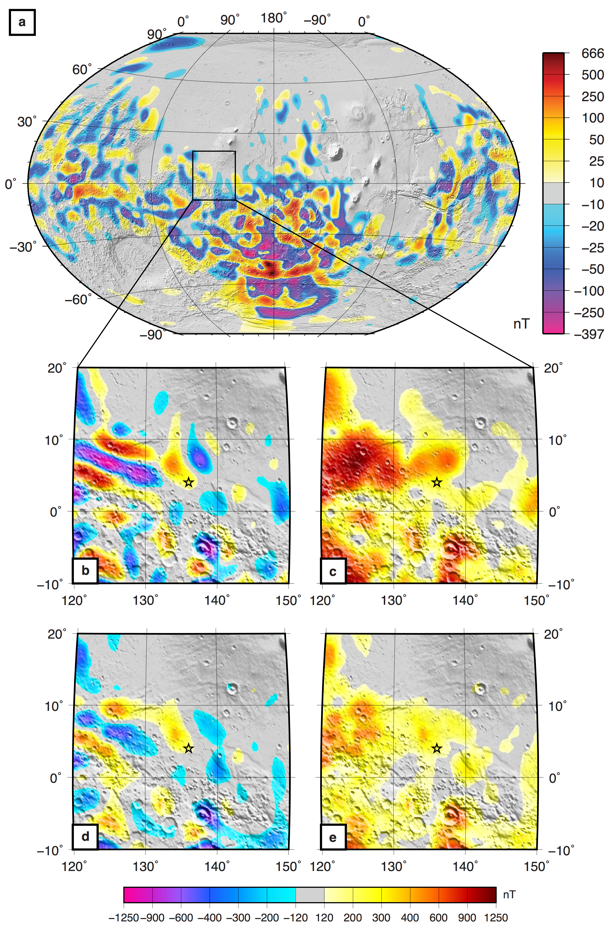
\includegraphics[width=0.8\textwidth]
{figures/Fig_6Sue.png}
\caption{(a) The radial component of the magnetic field 185 km above the planetary surface predicted by the model of \citep{Morschhauser2014}. The model uses MGS data only.  The insets (b)-(e) show two higher resolution regional model predictions for the surface field in the vicinity of the InSight landing site \cite{Langlais2017, Mittelholz2017}. Insets (b) and (d) show the radial magnetic field, $B_{r}$, and (c) and (e) the amplitude of the magnetic field, $\vert$B|, for each model respectively.  Both models use the same equivalent source dipole modeling approach and use MAVEN and MGS data.  The model in (b, c) is extracted from a global solution, and the model in (d,e) is a local solution in the vicinity of the landing site – both models agree well in overall structure.}
\label{fig:Magneticfield} 
\end{center}
\end{figure}

